%\\\///\\\///\\\///\\\///\\\///\\\///\\\///\\\///\\\///\\\///\\\///\\\///\\\///\\\///\\\///\\\///\\\///\\\///\\\///
% \\//  \\//  \\//  \\//  \\//  \\//  \\//  \\//  \\//  \\//  \\//  \\//  \\//  \\//  \\//  \\//  \\//  \\//  \\//
%  \/    \/    \/    \/    \/    \/    \/    \/    \/    \/    \/    \/    \/    \/    \/    \/    \/    \/    \/
%
%       Projekt:        Bachelor Thesis
%       Autor:          Felix Dietze
%       Datum:          2011
%
%       Comment:        This is the main file
%
%  /\    /\    /\    /\    /\    /\    /\    /\    /\    /\    /\    /\    /\    /\    /\    /\    /\    /\    /\
% //\\  //\\  //\\  //\\  //\\  //\\  //\\  //\\  //\\  //\\  //\\  //\\  //\\  //\\  //\\  //\\  //\\  //\\  //\\
%///\\\///\\\///\\\///\\\///\\\///\\\///\\\///\\\///\\\///\\\///\\\///\\\///\\\///\\\///\\\///\\\///\\\///\\\///\\\

% Syntax: "\documentclass[parameter]{class}
% class: book, report, article, letter or slides
% parameter:
%       10pt | 11pt | 12pt      ~ reference value for the font size
%       oneside | twoside       ~ ..well..
%       fleqn                   ~ formulas appear left-aligned (and not centered as by default)
\documentclass[12pt,twoside,a4paper]{book}

% ========================================================================================== additional packages \/

\usepackage[utf8]{inputenc}
\usepackage{a4}         % Standard is "letter"..we want DIN A4
\usepackage{fancyhdr}   % The best package for decorating latex-documents
\usepackage{german}     % This work is in german..and everything we need for this language is in this package
\usepackage{makeidx}    % For creating the index
\usepackage{nomencl}		% Nomenclature package; formats glossary entries to show
\usepackage{color}			% Color-package
\usepackage{t1enc}			% Now we can use german letters in the "\hyphenation" - command
\usepackage{latexsym}		% Now we can use different math. symbols
\usepackage{wrapfig}		% Using for the \wrapfigure - environment to wrap text around graphics
\usepackage{amsthm}			% Now we can use \theormstyle
\usepackage{amssymb}   % AMS symbol fonts for LaTeX.

\usepackage{graphicx}
\usepackage{pslatex}
\usepackage{ifthen}

\usepackage[T1]{fontenc}
\usepackage{pslatex}

%extern packages
%\usepackage{packages/ushort}
\usepackage{psfrag}
\usepackage{subfigure}

% \usepackage{amsfonts}  % TeX fonts from the American Mathematical Society.
% \usepackage{array}     % Arrays and tables with formatted columns.
% \usepackage{enumerate} % Adds an optional argument to the enumerate-env. which det. the style of the counter.
% \usepackage{eepic}     % Extensions to epic and the LaTeX drawing tools
% \usepackage{epic}      % Apackage enhancing LaTeX's picture mode
% \usepackage{ifthen}    % Conditionals in LaTeX2e documents.
% \usepackage{longtable} % Support for tables longer than a page.
% \usepackage{theorem}   % An extension to "\newtheorem"-structure%\usepackage{packages/mm}% ???

\usepackage{listings}  % Typeset source code listings using LaTeX.
\lstloadlanguages{C++}
\lstset{language=C++}

% \usepackage[dvips]{graphicx}
% \usepackage{wrapfig}
% \usepackage{psfrag}
% \usepackage{amsthm}
% \usepackage{amssymb}
% \usepackage{url}
% \usepackage{alltt}


% ================================================================================================ preprocessing \/

% ============================================================ style definitions and declarations \/

%%%
% Footer and header
%%%
\setlength{\headheight}{14.5pt}
\addtolength{\headwidth}{0.5\marginparwidth}
\lhead[\fancyplain{}{\thepage}]{\fancyplain{}{\nouppercase{\sffamily\rightmark}}}
\rhead[\fancyplain{}{\nouppercase{\sffamily\leftmark}}]{\fancyplain{}{\thepage}}

%%%
% Hyphenation
%%%
\hyphenation{FAVOuR quader-förmige}


% ================================================================================== new commands \/

%%%
% Adding a completely blank page (no footer, no header)
%%%
\newcommand{\blankpage}
{
  \clearpage{\pagestyle{empty}\cleardoublepage}
}

%%%
% Graphicspath (not needed yet)
%%%
\graphicspath{
	{pictures/}
}

%%%
% New commands for including graphics
%%%
\setlength{\fboxsep}{0.3cm}		% Separation between the framebox and the room inside !
\newlength{\gw}					% New lentgh for the width of the graphic !

\newcommand{\graphik}[2][1]{\includegraphics[width=#1\gw]{#2}}

\newcommand{\rahmengraphik}[2][1]
{
	\setlength{\gw}{#1\textwidth}
	\addtolength{\gw}{-2\fboxsep}
	\addtolength{\gw}{-2\fboxrule}
	\centering
        \graphik{#2}
%%	\framebox[#1\textwidth]{\graphik{#2}}
}

%%%
% Listingsdefinitions
%%%

\definecolor{black_color}{rgb}{0.0,0.0,0.0}
\definecolor{listingbgr_color}{rgb}{1.0,1.0,0.9}
\lstset{basicstyle=\small}
\lstset{stringstyle=\ttfamily}
\lstset{backgroundcolor=\color{listingbgr_color}}
\lstset{framesep=0.3cm}
\lstset{frame=single}
\lstset{captionpos=b}
\lstset{tabsize=2}
\lstset{abovecaptionskip=0.5cm}
\renewcommand{\lstlistlistingname}{Listingsverzeichnis}

%%%
% We want also subsubsections to be enumerated
%%%
\setcounter{secnumdepth}{3}
\setcounter{tocdepth}{3}


%%%
% Prepare the environment for definitions
%%%
\theoremstyle{definition}
\newtheorem{definition}{Definition}[chapter]
\newtheorem{theorem}{Satz}[chapter]


\makeglossary
%\makeindex

% ==================================================================================================== main part \/
\begin{document}

% ======================================================================= FRONT PART OF THE BOOK \/
\frontmatter

% ============================================================================== titel \/
%\\\///\\\///\\\///\\\///\\\///\\\///\\\///\\\///\\\///\\\///\\\///\\\///\\\///\\\///\\\///\\\///\\\///\\\///\\\///
% \\//  \\//  \\//  \\//  \\//  \\//  \\//  \\//  \\//  \\//  \\//  \\//  \\//  \\//  \\//  \\//  \\//  \\//  \\//
%  \/    \/    \/    \/    \/    \/    \/    \/    \/    \/    \/    \/    \/    \/    \/    \/    \/    \/    \/
%
%       Projekt:        Bachelor Thesis
%       Autor:          Felix Dietze
%       Datum:          2011
%
%       Comment:        Here is the definition of the titlepage
%
%  /\    /\    /\    /\    /\    /\    /\    /\    /\    /\    /\    /\    /\    /\    /\    /\    /\    /\    /\
% //\\  //\\  //\\  //\\  //\\  //\\  //\\  //\\  //\\  //\\  //\\  //\\  //\\  //\\  //\\  //\\  //\\  //\\  //\\
%///\\\///\\\///\\\///\\\///\\\///\\\///\\\///\\\///\\\///\\\///\\\///\\\///\\\///\\\///\\\///\\\///\\\///\\\///\\\

\begin{titlepage}

\begin{center}

\parbox{8cm}{
\includegraphics[height=1.6cm]{title/logo_rwth_color}}
\hfill
\parbox{2.5cm}{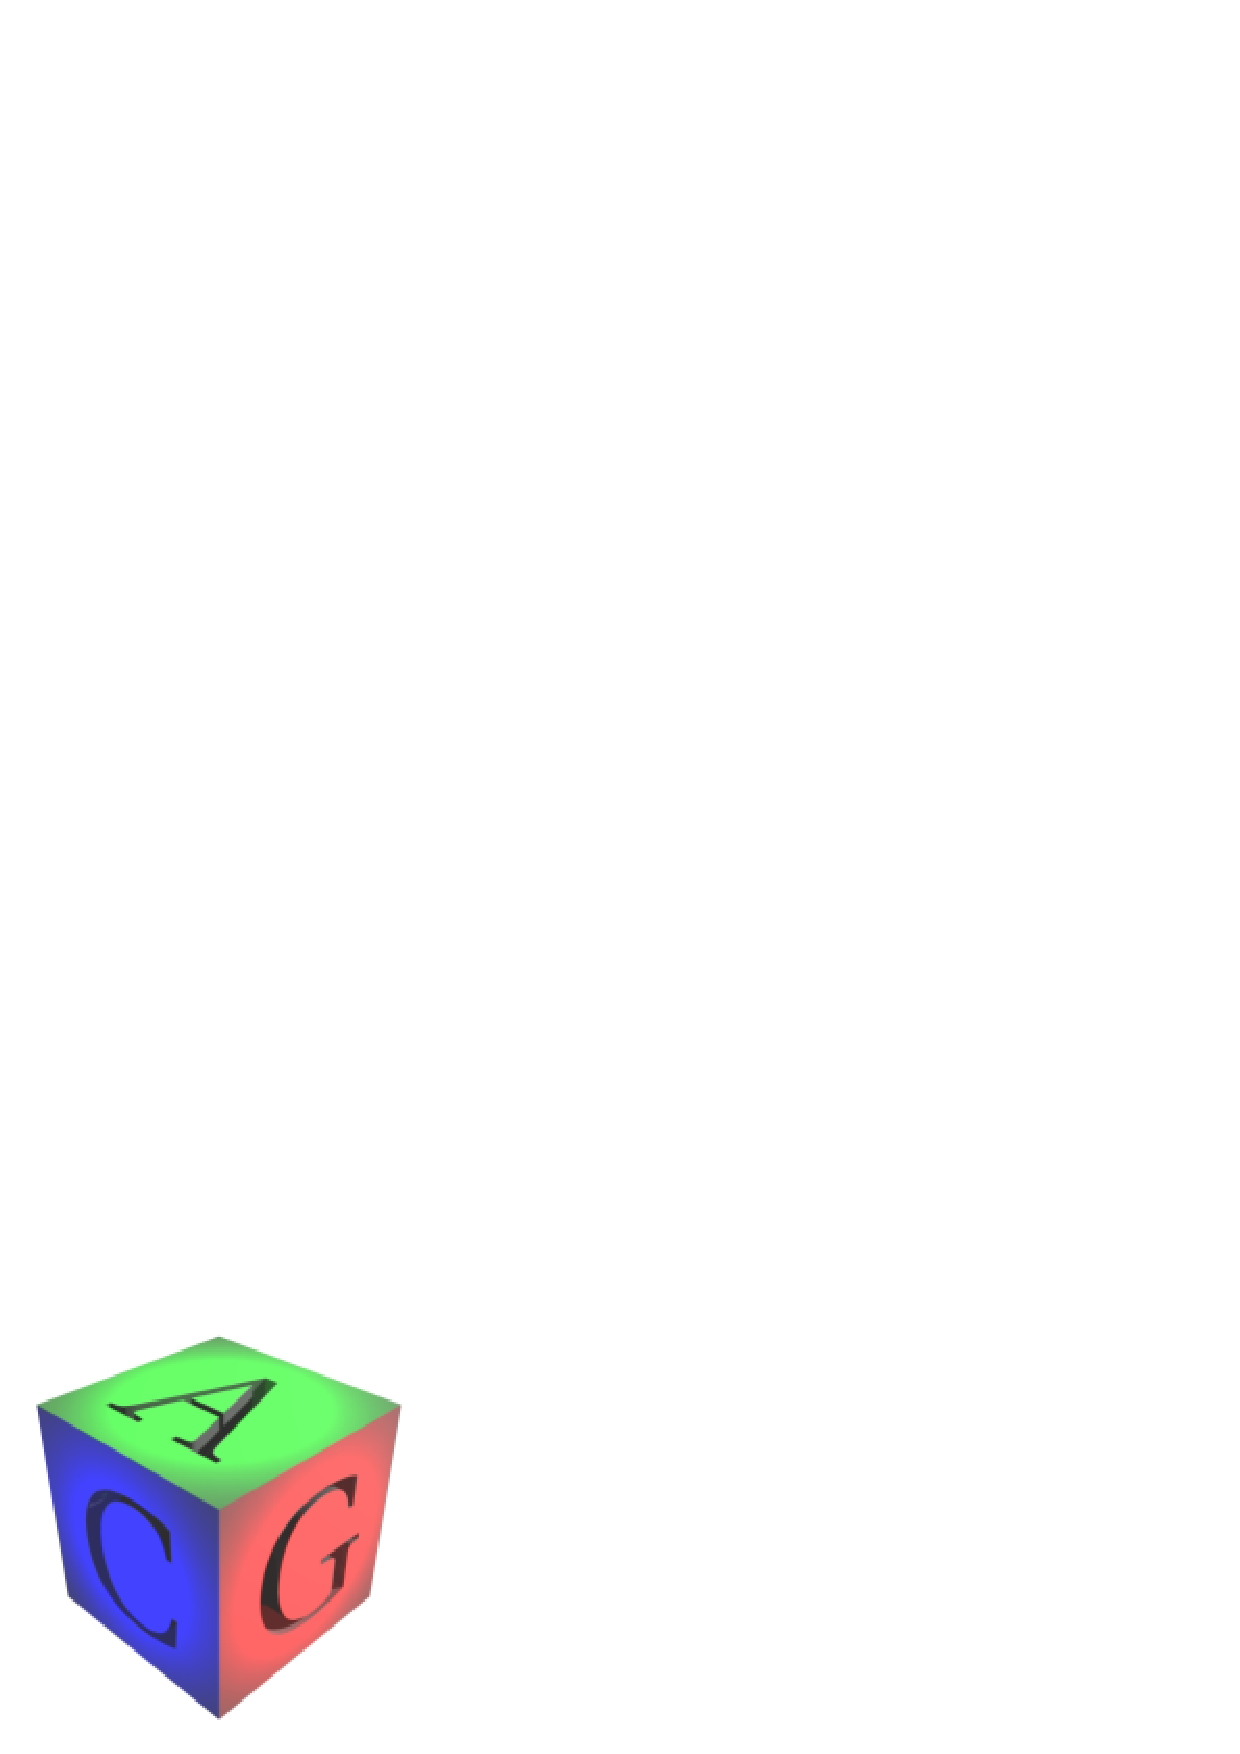
\includegraphics[width=2.3cm]{title/logo_acg_color}}

\vspace{0.5cm}

\vspace{0.75cm}

\textsf
{
Fakultät für Mathematik, Informatik und Naturwissenschaften\\
Lehrstuhl für Informatik VIII (Computergraphik und Multimedia)\\
Prof. Dr. Leif Kobbelt
}

\rule{\linewidth}{1pt}

\vspace{1.75cm}
\LARGE
\textbf{Bachelorarbeit}

\vspace{1.7cm}
\huge
Vorhersage und Interaktive Komposition von Noise-Funktionen zum Rendern Unbeschränkter Prozeduraler Welten in Echtzeit

\vspace{2.0cm}
\Large
Felix Dietze\\
\large
Matrikelnummer: 290734

\vspace{0.5cm}
August 2011

\vspace{1.05cm}
\rule{\linewidth}{1pt}

\vspace{0.5cm}
\textsf{\textbf{
\normalsize
\begin{tabular}{ll}
Erstgutachter:  & Prof. Dr. Leif Kobbelt\\
Zweitgutachter: & xxxxxxxxxxxxx\\
\end{tabular}
}}
\end{center}

\end{titlepage}


% ========================================================================= empty page \/
% \blankpage

% ==================================================================== acknowledgement \/
% \include{acknowledgement}

% ========================================================================= empty page \/
\blankpage

% ========================================================================= dedication \/
%\include{dedication}

% ========================================================== Eidesstattliche Erklärung \/
%\\\///\\\///\\\///\\\///\\\///\\\///\\\///\\\///\\\///\\\///\\\///\\\///\\\///\\\///\\\///\\\///\\\///\\\///\\\///
% \\//  \\//  \\//  \\//  \\//  \\//  \\//  \\//  \\//  \\//  \\//  \\//  \\//  \\//  \\//  \\//  \\//  \\//  \\//
%  \/    \/    \/    \/    \/    \/    \/    \/    \/    \/    \/    \/    \/    \/    \/    \/    \/    \/    \/
%
%	Projekt:	Bachelor Thesis
%	Autor:	    Felix Dietze
%	Datum:		2011
%
%	Comment:	Affirmation
%
%  /\    /\    /\    /\    /\    /\    /\    /\    /\    /\    /\    /\    /\    /\    /\    /\    /\    /\    /\
% //\\  //\\  //\\  //\\  //\\  //\\  //\\  //\\  //\\  //\\  //\\  //\\  //\\  //\\  //\\  //\\  //\\  //\\  //\\
%///\\\///\\\///\\\///\\\///\\\///\\\///\\\///\\\///\\\///\\\///\\\///\\\///\\\///\\\///\\\///\\\///\\\///\\\///\\\

\pagestyle{fancyplain}

\begin{figure}
I hereby affirm that I composed this work independently and used no other than the specified sources and tools and
that I marked all quotes as such.
\bigskip

Hiermit versichere ich, diese Arbeit selbst\"andig verfasst und keine anderen als die angegebenen Quellen und
Hilfsmittel benutzt, sowie Zitate kenntlich gemacht zu haben.
\medskip

\begin{flushright}
Aachen, den \today

\vspace{1.5cm}
\small
(Felix Dietze)
\end{flushright}
\end{figure}

%\clearpage
%\thispagestyle{empty}
%\ \\[3cm]
%\begin{center}
%\parbox{10cm}
%{ 
%Eidessstattliche Erklärung: \newline\newline
%Ich versichere, dass ich die vorliegende Arbeit selbständig verfaßt und keine anderen als die angegebenen
%Quellen und Hilfmittel benutzt habe.
%\\[8mm] 
%Aachen, den \today
%}
%\end{center}


% ========================================================================= empty page \/
\blankpage

% =========================================================================== CONTENTS \/
{ % changing "parskip" only here
% \setlength{\parskip}{0.2ex plus0.1ex minus0.1ex}

\pagestyle{fancyplain}
\tableofcontents
\newpage

% \listoffigures
% \addcontentsline{toc}{chapter}{Abbildungsverzeichnis}
% 
% \listoftables
% \addcontentsline{toc}{chapter}{Tabellenverzeichnis}
% 
% \lstlistoflistings
% \addcontentsline{toc}{chapter}{Listingsverzeichnis}
}

% ======================================================================== MAIN PART OF THE BOOK \/
\mainmatter

\chapter*{Einleitung}
%%\begin{figure}[ht!]
%%\rahmengraphik[0.5]{01/bla.eps}
%%\caption{ Beispiel }
%%\label{bsp_label}
%%\end{figure}

% ========================================================================= empty page \/
\blankpage

% Footer and header extra for introduction
% \lhead[\fancyplain{}{\thepage}]{\fancyplain{}{\nouppercase{\sffamily Einleitung}}}
% \rhead[\fancyplain{}{\nouppercase{\sffamily Einleitung}}]{\fancyplain{}{\thepage}}

% \addcontentsline{toc}{chapter}{Einleitung}
% \include{chapters/00_introduction}

% Footer and header back to standard
% \lhead[\fancyplain{}{\thepage}]{\fancyplain{}{\nouppercase{\sffamily\rightmark}}}
% \rhead[\fancyplain{}{\nouppercase{\sffamily\leftmark}}]{\fancyplain{}{\thepage}}

% \include{chapters/01_meshreconstruction}
% \include{chapters/02_poly}
% \include{chapters/03_volume}
% \include{chapters/04_polyagain}
% \include{chapters/05_outputoptimization}
% \include{chapters/06_conclusions}

% ======================================================================== BACK PART OF THE BOOK \/
\backmatter

% =========================================================================== glossary \/

% % Footer and header extra for glossary
% \lhead[\fancyplain{}{\thepage}]{\fancyplain{}{\nouppercase{\sffamily Glossar}}}
% \rhead[\fancyplain{}{\nouppercase{\sffamily Glossar}}]{\fancyplain{}{\thepage}}
% 
% \addcontentsline{toc}{chapter}{Glossar}
% \def\nomlabel#1{\sffamily\bfseries#1\hfil}
% \renewcommand{\nomname}{Glossar}
% \printglossary[1.5cm]
% 
% % Footer and header back to standard
% \lhead[\fancyplain{}{\thepage}]{\fancyplain{}{\nouppercase{\sffamily}}}
% \rhead[\fancyplain{}{\nouppercase{\sffamily}}]{\fancyplain{}{\thepage}}

% ========================================================================= literature \/
\bibliographystyle{alpha}
\bibliography{bachelorthesis}
\nocite{*}

% ============================================================================== index \/
%\printindex

\end{document}
